%%%%%%%%%%%%%%%%%%%%%%%%%%%%%%%%%%%%%%%%%
% Short Sectioned Assignment LaTeX Template Version 1.0 (5/5/12)
% This template has been downloaded from: http://www.LaTeXTemplates.com
% Original author:  Frits Wenneker (http://www.howtotex.com)
% License: CC BY-NC-SA 3.0 (http://creativecommons.org/licenses/by-nc-sa/3.0/)
%%%%%%%%%%%%%%%%%%%%%%%%%%%%%%%%%%%%%%%%%

%----------------------------------------------------------------------------------------
%	PACKAGES AND OTHER DOCUMENT CONFIGURATIONS
%----------------------------------------------------------------------------------------

\documentclass[paper=a4, fontsize=11pt]{scrartcl} % A4 paper and 11pt font size

% ---- Entrada y salida de texto -----

\usepackage[T1]{fontenc} % Use 8-bit encoding that has 256 glyphs
\usepackage[utf8]{inputenc}

% ---- Idioma --------

\usepackage[spanish, es-tabla]{babel} % Selecciona el español para palabras introducidas automáticamente, p.ej. "septiembre" en la fecha y especifica que se use la palabra Tabla en vez de Cuadro

% ---- Otros paquetes ----

\usepackage{amsmath,amsfonts,amsthm} % Math packages
\usepackage{graphics,graphicx, floatrow} %para incluir imágenes y notas en las imágenes
\usepackage{graphics,graphicx, float} %para incluir imágenes y colocarlas
\usepackage{hyperref} % url in references
\usepackage{textcomp}
\usepackage{listings}
\usepackage{titlesec}

% Para hacer tablas comlejas
\usepackage{multirow}
\usepackage{threeparttable}

\usepackage{fancyhdr} % Custom headers and footers
\pagestyle{fancyplain} % Makes all pages in the document conform to the custom headers and footers
\fancyhead{} % No page header - if you want one, create it in the same way as the footers below
\fancyfoot[L]{} % Empty left footer
\fancyfoot[C]{} % Empty center footer
\fancyfoot[R]{\thepage} % Page numbering for right footer
\renewcommand{\headrulewidth}{0pt} % Remove header underlines
\renewcommand{\footrulewidth}{0pt} % Remove footer underlines
\setlength{\headheight}{13.6pt} % Customize the height of the header

\numberwithin{equation}{section} % Number equations within sections (i.e. 1.1, 1.2, 2.1, 2.2 instead of 1, 2, 3, 4)
\numberwithin{figure}{section} % Number figures within sections (i.e. 1.1, 1.2, 2.1, 2.2 instead of 1, 2, 3, 4)
\numberwithin{table}{section} % Number tables within sections (i.e. 1.1, 1.2, 2.1, 2.2 instead of 1, 2, 3, 4)

\setlength\parindent{0pt} % Removes all indentation from paragraphs - comment this line for an assignment with lots of text

\newcommand{\horrule}[1]{\rule{\linewidth}{#1}} % Create horizontal rule command with 1 argument of height

\usepackage{textcomp}
\usepackage{listings}
\usepackage{color}

\definecolor{mygreen}{rgb}{0,0.6,0}
\definecolor{mygray}{rgb}{0.5,0.5,0.5}
\definecolor{mymauve}{rgb}{0.58,0,0.82}


\lstdefinestyle{C}{
    backgroundcolor=\color{white},
    basicstyle=\footnotesize\ttfamily,
    breakatwhitespace=false,
    breaklines=true,  
    captionpos=b,
    commentstyle=\color{mygreen},
    extendedchars=true,
    frame=single,
    keepspaces=true,
    keywordstyle=\color{blue},
    language=C,
    numbers=left,
    numbersep=5pt,
    numberstyle=\tiny\color{mygray},
    rulecolor=\color{black},
    showspaces=false,
    showstringspaces=false,
    showtabs=false,
    stringstyle=\color{mymauve},
    tabsize=2,
    title=\lstname
}

\lstdefinestyle{pseudo} {
	basicstyle=\scriptsize,
	language=C
}

%----------------------------------------------------------------------------------------
%	DATOS
%----------------------------------------------------------------------------------------

\newcommand{\myName}{Francisco Javier Bolívar Lupiáñez}
\newcommand{\myDegree}{Grado en Ingeniería Informática}
\newcommand{\myFaculty}{E. T. S. de Ingenierías Informática y de Telecomunicación}
\newcommand{\myDepartment}{Lenguajes y Sistemas de Información}
\newcommand{\myUniversity}{\protect{Universidad de Granada}}
\newcommand{\myLocation}{Granada}
\newcommand{\myTime}{\today}
\newcommand{\myTitle}{Trabajo propuesto}
\newcommand{\mySubtitle}{Tipo de schedule en parallel for de OpenMP}
\newcommand{\mySubject}{Programación Paralela}
\newcommand{\myYear}{2015-2016}

%----------------------------------------------------------------------------------------
%	PORTADA
%----------------------------------------------------------------------------------------


\title{	
	\normalfont \normalsize 
	\textsc{{\bf \mySubject \space (\myYear)} \\ \myDepartment} \\[20pt] % Your university, school and/or department name(s)
	\textsc{\myDegree \\[10pt] \myFaculty \\ \myUniversity} \\[25pt]
	\horrule{0.5pt} \\[0.4cm] % Thin top horizontal rule
	\huge \myTitle: \mySubtitle \\ % The assignment title
	\horrule{2pt} \\[0.5cm] % Thick bottom horizontal rule
	\normalfont \normalsize
}

\author{\myName} % Nombre y apellidos

\date{\myTime} % Incluye la fecha actual
%----------------------------------------------------------------------------------------
%	INDICE
%----------------------------------------------------------------------------------------

\begin{document}
	
\setcounter{page}{0}

\maketitle % Muestra el Título
\thispagestyle{empty}

\newpage %inserta un salto de página

\tableofcontents % para generar el índice de contenidos

\newpage

%----------------------------------------------------------------------------------------
%	DOCUMENTO
%----------------------------------------------------------------------------------------

\section{Planteamiento del problema}

Considerar el siguiente bucle: 
\begin{lstlisting}[style=pseudo]
for (i = 0; i < N; i++)
	f(i);
\end{lstlisting}
en el que el tiempo de ejecución de la función f() depende de la iteración i. Paraleliza el bucle anterior con una directiva \texttt{parallel for}. Realizar ejecuciones en las que se varíen el número de threads y en las que se modifiquen el tipo de \texttt{schedule} a \texttt{static}, \texttt{dynamic}, \texttt{guided}. Comprobar cómo se modifica el tiempo de ejecución en cada caso.

\section{Análisis}

El problema que se plantea es el de qué reparto es el más apropiado para aquellos algoritmos en los que todas las tareas no tienen el mismo costo computacional.
\\ \\
En OpenMP se puede controlar este reparto de la directiva \texttt{parallel for} con los distintos tipos de \texttt{schedule} y el tamaño de bloque que se utilizará.

\begin{itemize}
	\item \texttt{static}: El reparto se hace en tiempo de compilación y siempre será el mismo. Las iteraciones se dividen en bloques que se asignan en round-robin a las hebras: Por ejemplo si se tienen 8 iteraciones, 3 hebras y un tamaño de bloque de 2, este sería el reparto:
	\begin{itemize}
		\item P0: 0, 1, 6
		\item P1: 2, 3, 7
		\item P2: 4, 5
	\end{itemize}
	\item \texttt{dynamic}: El reparto se hace en tiempo de ejecución. Cada vez que una hebra realiza una tarea coge otra de la cola de trabajos. El tamaño de bloque por defecto es 1. El funcionamiento añade una sobrecarga a tener en cuenta.
	\item \texttt{guided}: Similar a \texttt{dynamic}, pero el tamaño de bloque empieza siendo grande y va reduciéndose. El tamaño de bloque se calcula como \textit{iteraciones restantes / número de hebras}, nunca siendo más pequeño que el tamaño de bloque que se le pasa como parámetro. Al igual que \texttt{dynamic} tiene sobrecarga adicional, pero menor para el mismo tamaño de bloque.
\end{itemize}

Se espera, por tanto, que el reparto \texttt{static} con bloques de N / P unidades sea el que peor resultados de, mientras que el uso de bloques de tamaño 1 se aproximará a los resultados obtenidos con \texttt{dynamic} y \texttt{guided} que obtendrán resultados similares, aunque tal vez el \texttt{guided} sea el que obtenga los mejores por tener una sobrecarga menor que el \texttt{dynamic}.

\section{Implementación}

\lstinputlisting[style=C]{codigo/main.cpp}

\section{Resultados}

Para tomar tiempos se ha utilizado un portátil \textit{MSI CX61 2PC} con las siguientes características:
\begin{itemize}
	\item \textbf{Procesador}: Intel\textregistered{} Core\texttrademark{} i7-4712MQ CPU @ 2.30GHz
	\item \textbf{Tamaño de caché}: 6MB
	\item \textbf{Memoria RAM}: 8GB
	\item \textbf{S.O.}: Linux Mint 17.3 "Rosa" - Cinnamon (64-bit)
	\item \textbf{Versión g++}: 4.8.4
	\item \textbf{Versión OpenMP}: 3.1
\end{itemize} 

Se ha lanzado el programa para cuatro hebras OpenMP y tamaños de 50.000 a 100.000 avanzando de 10.000 en 10.000.

\begin{center}
\begin{tabular}{ | c | c c c c | }
	\hline 
	N		&	Static (bloques)	&	Static (cíclico)	&	Dynamic		&	Guided		\\
	\hline
	50000	&	0,540194			&	0,314281			&	0,315153	&	0,313882	\\
	60000	&	0,801774			&	0,485337			&	0,452282	&	0,451983	\\
	70000	&	1,10983				&	0,772775			&	0,685909	&	0,683268	\\
	80000	&	1,42382				&	1,02538				&	0,920239	&	0,917319	\\
	90000	&	1,79697				&	1,33359				&	1,16581		&	1,16131		\\
	100000	&	2,2165				&	1,63686				&	1,44584		&	1,43517		\\
	\hline
\end{tabular}
\end{center}

\begin{figure}[H]
	\centering
	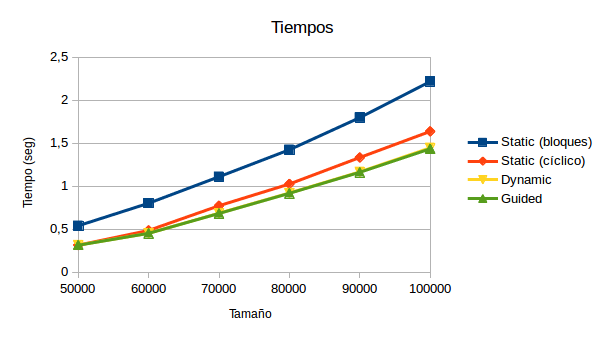
\includegraphics[width=12cm]{resultados/tiempos}
\end{figure}

\section{Conclusiones}

Como se esperaba, los mejores resultados se han obtenido usando \texttt{guided}, aunque la diferencia con \texttt{dynamic} es inapreciable. El reparto estático cíclico no trabaja del todo mal si se compara con el estático con bloques de tamaño N / P, pero sigue siendo peor que las dos alternativas mencionadas anteriormente.

\end{document}